% !Mode:: "TeX:UTF-8"
% !TEX root = ../main.tex
\chapter{非稳态层流流动的数值模拟方法}

\section{计算流体力学的研究方法}

%流体力学的研究方法

对于简单的流动问题,通过求解流体力学方程可以得到解析解,已知的解析解可以加深对流动机理的理解,但却很难直接用于工程分析和设计中。根据实际问题对方程进行简化并使用量纲分析来求解问题是一种可行的方法,主要适用于所研究的系统仅有一两个无量纲参数的情形。如果无量纲化的纳维尔-斯托克斯方程仅以雷诺数为独立参数,就常常使用这种方法。如果几何体的形状是固定不变的,我们可以通过相似模型实验得到想要的结果。时至今日,这种方法在实际工程设计中依然很有价值。问题在于,许多流动都需要若干个无量纲参数,可能无法建立起与实际流动相似的实验条件。例如,在飞机机翼的绕流中,为了利用更小的模型达到相同的雷诺数,就必须提高空气的流速,这可能会导致马赫数过高,为了避免这样的问题就要寻找合适的流体。在船只绕流问题中,同时满足雷诺数和弗劳德数也是几乎不可能的。与此同时,有的实验可能需要很高的成本。

随着电子计算机的诞生,计算的方法成为可能;随着计算机性能的提升和成本的下降,计算的手段也更加简易而高效。用计算机求解流体力学方程变得越来越重要,同时更多的人员使用这一方法研究流动现象,从而形成了计算流体力学这一研究领域。流动现象是用偏微分方程描述的,为了得到方程的数值解,使用离散方法将微分方程近似为代数方程然后求解,解的精度则取决于所使用的离散方法。

一个完整的数值方法应该从以下几个方面进行考虑。

(1)数学模型。包括偏微分方程和边界条件的建立。针对要解决的具体问题,选择合适的控制方程,这样的模型可能是对原始守恒方程作出一定的简化得到的。一种求解方法是针对一类特定的问题而提出来的,试图寻找可以求解所有流动问题的通用方法是不现实的;与此同时,适用性广的方法通常针对性较差,即在求解具体问题上不是最优的。

(2)离散方法。选择合适的离散方法对时间和空间进行离散,用得到的代数方程代替原来的微分方程。几种主要的方法是有限差分法(finite difference, FD)、有限体积法(finite volume, FV)和有限元法(finite element, FE)。谱方法(spectral scheme)、边界元法(boundary element)和元胞自动机(cellular automata)等其他方法适用于一些特殊的问题。

(3)坐标系和基向量的选取。流体力学的控制方程在不同的坐标系下具有不同的书写形式,例如直角坐标系、柱坐标系或球坐标系,正交或非正交坐标系下的表达方式也不相同。针对具体的流动选择合适的坐标系,这可能影响到离散方法和网格类型的选择。基向量的选择决定了向量和张量的定义,例如固定或可变、协变或逆变。速度向量和应力张量根据各坐标轴分解为各自的分量。

(4)网格划分。将问题所在的几何区域离散化处理,所有的变量就定义在这些离散后的位置上,最终目的是得到这些位置上各个变量的值。经过离散化处理,原先的求解区域被划分为大量的小区域。划分后的每个小区域——或称为网格——主要有以下几种形式。

\begin{enumerate}
	\item 结构化网格(structured grid)。
	\item 分块结构化网格(block-structured grid)。
	\item 非结构化网格(unstructured grid)。
\end{enumerate}

(5)有限近似。在离散化过程中需要选择近似的程度。有限差分方法中要选择网格点处导数的近似,有限体积方法中要选择面积分和体积分的近似,有限元方法中则要选择形状函数和权重函数。近似方法的选择影响到计算的精度,也影响到求解的困难程度、程序编写调试的难度以及程序运行的速度。最终需要在简单易行、精度和计算效率之间取得平衡。

(6)求解方法。离散之后的方程通常是一个庞大的非线性代数方程组。对于非稳态流动,通常像常微分方程的初值问题那样来求解。每经过一个时间步长都去求解一个椭圆形问题。稳定流动问题通常采用伪时间推进(pseudo-time marching)或一种等效迭代方法(?equivalent iteration scheme)。由于方程是非线性的,所以要用迭代的方法求解。这些方法对方程进行线性化,得到的线性方程组几乎总是可以用迭代的技术进行求解。求解方法的选择取决于网格的类型和每一个线性方程中节点的数目。

(7)收敛标准。对于迭代方法,要设置一个收敛的标准。通常情况下有两种迭代的级别:求解线性方程过程中的内部迭代和处理方程组之间的耦合及非线性关系过程中的外部迭代。无论是从精度还是效率的角度,迭代过程的终止条件都十分重要。

数值解法应当具有某些性质,大多数情况下不可能分析出完整的解方法,如果方法中的某一个环节不满足解的性质,那整个方法也不满足。以下是一些重要的性质。

(1)一致性。当网格间距趋向于零时,离散化应当变得精确。离散方程和真实方程之间的差距称为截断误差(truncation error),通常用泰勒级数在某个节点上展开的值与真实值的差来表示。当网格尺寸 $\Delta t \to 0$ 和/或 $\Delta x_i \to 0$ 时,具有一致性的方法应当使得截断误差为零。截断误差通常和网格尺寸 $\Delta x_i$ 和/或时间步长 $\Delta t$ 成正比,如果截断误差的主要项正比于 $(\Delta x_i)^n$ 或 $(\Delta t)^n$,则称为 $n$ 阶近似($n>0$)。%有些离散方法使截断误差成为 $\Delta x_i$ 和 $\Delta t$ 之比的函数,一致性的要求变成了:

即使解方法具有一致性,也不意味着离散方程组的解在小步长的极限下成为微分方程的解,因为解还需要具有稳定性。

(2)稳定性。解的稳定性要求它在求解过程中不会放大误差。对时间问题,稳定性保证了当实际解有边界时数值解也有边界。对迭代方法而言,稳定解意味着不会发散。稳定解不容易判断,尤其是当存在边界条件和非线性的时候。因此,常常在具有常系数、不含边界条件的线性问题时去验证稳定性。经验表明,用这种方式得到的结果通常可以用于更复杂的情况,除了部分例外。广泛采用的研究稳定性的方法是冯纽曼法(von Neumann's method)。

(3)收敛性。随着网格尺寸趋于零,离散方程的解趋于实际微分方程的解的时候,该方法具有收敛性。对于线性初值问题,Lax 等价理论(Lax equivalence theorem)\cite{}指出,给定一个合适的线性初值问题和有限差分近似,并且满足一致性条件,那么稳定性就成为收敛性的充要条件。对于受边界条件影响的非线性问题,稳定性和收敛性都难以验证。因此,收敛性通常使用数值实验来检验,例如,用一系列连续变化密度的网格重复计算,如果方法是稳定的并且离散过程中近似方法也都保持一致,最终的解就会收敛于一个网格无关的解。

(4)守恒性。求解的方程满足守恒率,相应的数值方法也同样应该满足。在稳定状态且不存在源和汇的情况下,离开一个控制体的守恒量等于进入这个控制体的量。如果对方程的守恒形式使用有限体积法,那么每一个小的控制体和整个求解区域都要满足守恒率。源和汇的处理应该是一致的,以使得整个区域内源和汇的代数和等于守恒量通过边界的净流率。守恒性是解方法的一个重要性质,因为它为解的误差强加了一个限制。如果质量守恒、动量守恒和能量守恒得不到保证,就会人为产生源和汇,改变局部和整体的平衡。

(5)有界性。数值解应该具有一定的边界,有的物理量不能取负值(例如密度、动能),有的量必须介于 0\% 和 100\% 之间(例如浓度);不存在源和汇时,一些方程要求物理量的最大最小值应在区域的边界上取得。数值解法应该考虑这些条件。有界性难以得到保证。仅有一阶格式可以保证这个性质,所有的高阶格式都会产生超出边界的解,但是这仅会在网格过于稀疏时发生。

(6)可实现性。过于复杂而无法直接处理的模型应该保证可以得到物理上真实的解。这并不是一个数值自身的问题,而是非现实的模型可能产生出非物理的解,或者造成数值方法的发散。

(7)准确性。数值解均为近似解,除了求解算法的误差、程序或边界条件的误差外,通常还包含三种误差:模型误差、离散误差和迭代误差。模型误差为实际流动和数学模型真实解之间的差距;离散误差为守恒方程真实解和离散之后得到的代数方程组真实解之间的差值;迭代误差为求解代数方程组时迭代得到的解和真实解之间的误差。有时,不同的误差可能相互抵消,因为如此,粗糙网格的误差可能比细密网格的误差更小。

通常使用的离散方法有有限差分、有限体积、有限单元法几种。

(1)有限差分法。有限差分是最早出现的求解偏微分方程的数值方法,被认为由欧拉于 18 世纪提出。求解开始于微分形式的守恒方程,求解区域划分为排列在一起的网格。在每一个网格点上,用函数在该节点的值代替该节点上的偏导数,微分方程得到近似。每个节点都将得到一个代数方程,该节点和邻近节点上的变量都作为未知变量而存在。原则上,有限差分法可以用于任何网格类型,但在实际中,它常被用于结构化网格。通常用泰勒级数展开或多项式拟合的方法得到变量的一阶和二阶导数,必要时,还可以用这些方法得到网格节点之外的其他节点上的变量值。对于结构化网格,有限差分法简单而有效,易于获得高阶格式,它的缺点在于守恒性不易实施,而且不适用于复杂的流动情形。

(2)有限体积法。有限体积法从积分形式的守恒方程开始,求解区域被划分为紧邻着的有限数量的控制体,在每一个控制体上应用守恒方程。每个控制体中心节点上的值待求,用插值的方法得到控制体每个面上的值(用中心节点的值表示),用合适的积分公式表示面积分和体积分,我们可以得到每个控制体上的代数方程,临近节点上的变量也出现在这个方程中。有限体积法适用于任何类型的网格,因此也适用于复杂的几何区域。网格仅定义了几何区域的边界,并且不需要和坐标系联系起来。只要具有同一边界的控制体具有相同的面积分,该方法就满足守恒性。有限体积法易于理解和编程实现,缺点在于,与有限差分相比,二阶以上的格式在三维情形中难以实现。

(3)有限单元法。

\section{问题描述}

\subsection{控制方程} % homogenous fluid region, and porous region

\subsection{边界条件} % Including interface between the homogeneous fluid and porous medium regions

\section{数值方法}

\subsection{时间和空间的离散方法}

\subsection{求解器} % SIMPLE

\subsection{网格生成和网格独立性分析}

流动区域设定为边长 60 的正方形。为了获得圆柱内外的流动状态,流动区域被划分为三块,其中有两块位于圆柱内部,一块位于圆柱外部,见图~\ref{fig: grid}。网格尺寸见表~\ref{tab: grid}。雷诺数和达西数分别为 100 和 0.0001。
\begin{figure}
	\centering
	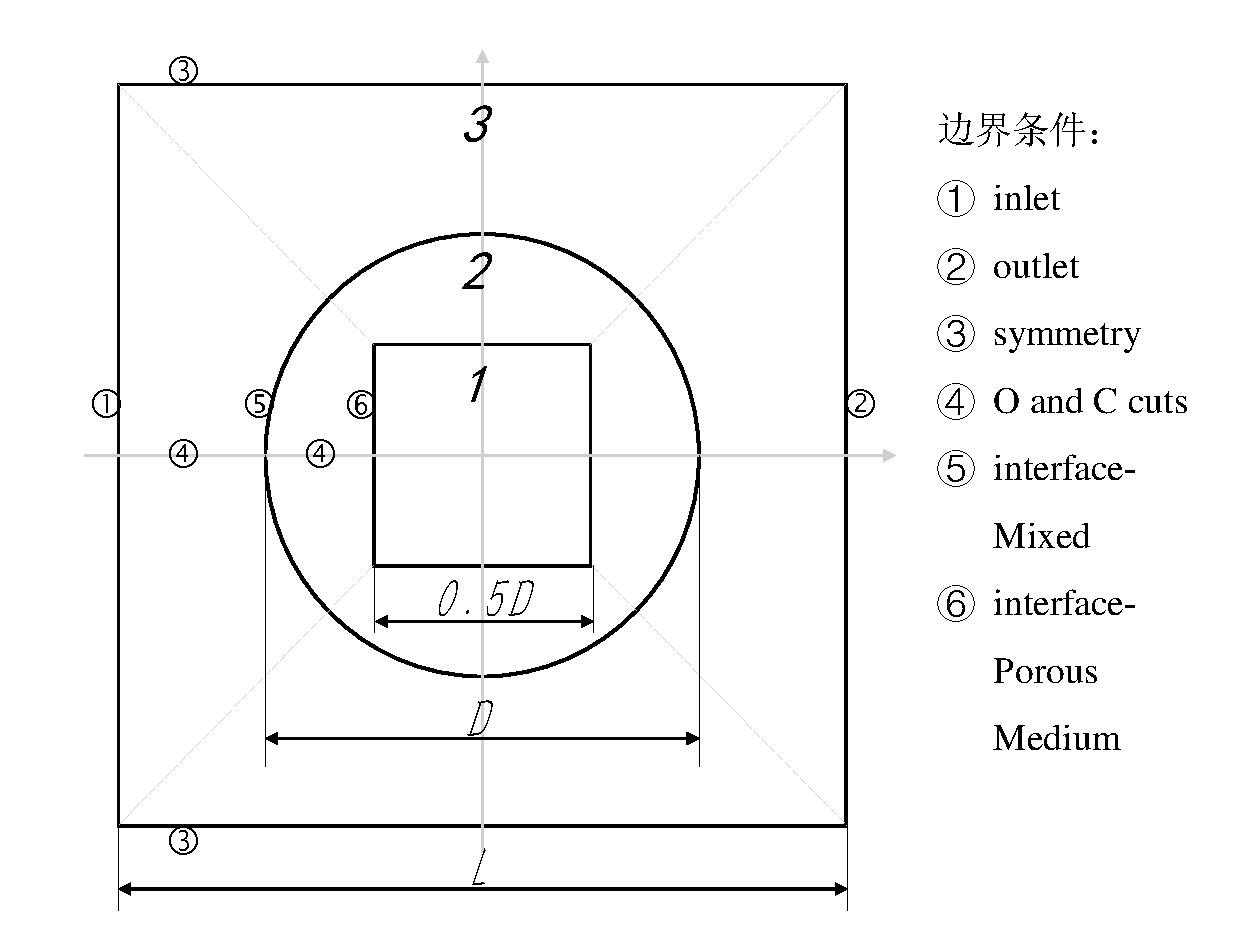
\includegraphics[scale=.6]{../diagrams/grid}
	\caption{网格划分}\label{fig: grid}
\end{figure}

\begin{table}
	\caption{网格尺寸}\label{tab: grid}
	\vspace{.5em}\centering\wuhao
	\begin{tabular}{ccccc}
		\toprule[1.5pt]
		\multirow{2}[3]{*}{序号} & \multicolumn{3}{c}{网格尺寸} & \multirow{2}[3]{*}{平均阻力系数} \\
		\cmidrule[.67pt](lr){2-4}
		& Block 1 & Block 2 & Block 3 & \\
		\midrule[1pt]
		1 & 40 $\times$ 40 & 160 $\times$ 25 & 160 $\times$ 140 & 1.2354 \\
		2 & 60 $\times$ 60 & 240 $\times$ 30 & 240 $\times$ 170 & 1.2426 \\
		3 & 80 $\times$ 80 & 320 $\times$ 40 & 320 $\times$ 200 & 1.2462 \\
		4 & 100 $\times$ 100 & 400 $\times$ 50 & 400 $\times$ 230 & 1.2417 \\
		\bottomrule[1.5pt]
	\end{tabular}
\end{table}

\section{本章小结}
